\chapter{บทนำ}
\label{chapter:introduction}

บริษัท วงใน มีเดีย จำกัด (สำนักงานใหญ่) เป็นองค์กรที่ให้บริการและดูแลเว็บไซต์ wongnai.com และแอปพลิเคชัน Wongnai บนโทรศัพท์มือถือทั้งบนระบบปฏิบัติการ Android และ iOS (ต่อจากนี้จะขอเรียกว่า Wongnai) ซึ่งที่รู้จักกันอย่างดีสำหรับบริการค้นหา-รีวิวร้านอาหารในประเทศไทย และเป็นแอปพลิเคชันแรก ๆ ของประเทศไทยที่ให้บริการในด้านนี้ ในช่วงแรกของ Wongnai นั้นมีจำนวนผู้ใช้งานน้อย แต่เนื่องด้วยการเข้ามาของสมาร์ทโฟน ทำให้จำนวนผู้งานเพิ่มขึ้นอย่างก้าวกระโดดเป็นอย่างมาก และปัจจุบัน Wongnai นอกจากจะให้บริการค้นหาและรีวิวร้านอาหารแล้ว ยังสามารถค้นหาที่พัก-ที่เที่ยว, ค้นหาสูตรอาหาร หรือแม้กระทั่งสั่งอาหารเดลิเวอรีก็สามารถทำได้

การโฆษณาถือว่าเป็นส่วนสำคัญอย่างยิ่งที่จะทำให้ผู้บริโภคสามารถรับรู้ถึงการมีตัวตนอยู่ของสินค้าและบริการ นอกจากการสร้างสรรค์โฆษณาให้ดูน่าสนใจแล้ว การเลือกตำแหน่งที่จะแสดงโฆษณาก็ถือว่าเป็นสิ่งที่สำคัญ เพื่อให้โฆษณาเข้าถึงกลุ่มเป้าหมายได้มากที่สุด

ปัจจุบัน Wongnai นั้น มีจำนวนผู้ใช้งานเยอะมากถึง 8 ล้านรายต่อเดือน ~\cite{wongnai} เนื้อหาหลักของ Wongnai เองก็เป็นเรื่องเกี่ยวกับอาหาร, ร้านอาหาร และร้านบริการอื่น ๆ เช่น ร้านเสริมสวย, ร้านนวด เป็นต้น Wongnai จึงนับว่าเป็นตัวเลือกที่ดีสำหรับการโฆษณาที่มีเนื้อหาเกี่ยวกับร้านอาหารและร้านบริการ

แต่เดิมแล้ว Wongnai สามารถแสดงร้านที่เป็นโฆษณาได้ตามช่วงเวลาที่ตกลงกับลูกค้าไว้ ซึ่งโฆษณาจะปรากฏอยู่ในตำแหน่งต่าง ๆ ของเว็บไซต์และแอปพลิเคชัน ดังรูปที่ 1.1
เพื่อเป็นการสร้างความเชื่อมั่นให้กับลูกค้าที่ต้องการจะลงโฆษณากับ Wongnai จึงจำเป็นต้องมีการพัฒนาระบบจัดการโฆษณาแบบใหม่ขึ้นมา โดยระบบนั้นสามารถแสดงโฆษณาโดยจำกัดจำนวนการคลิกและการแสดงโฆษณา ยกตัวอย่างเช่น โฆษณาหนึ่งถูกจำกัดการแสดงไว้ที่ 10,000 ครั้ง หากมีการแสดงโฆษณาครบ 10,000 ครั้งแล้ว ระบบก็จะนำโฆษณาออกโดยอัตโนมัติ หรือ โฆษณาหนึ่งถูกจำกัดการคลิกไว้ที่ 5,000 ครั้ง หากมีผู้ใช้คลิกเข้าไปที่โฆษณาครบ 5,000 ครั้งแล้ว ระบบก็จะนำโฆษณาออกโดยอัตโนมัติ วิธีการแสดงโฆษณาแบบใหม่จะทำให้ลูกค้าจะรู้สึกคุ้มค่ามากขึ้น เนื่องด้วยวิธีการแสดงโฆษณาแบบใหม่สามารถการันตีได้อย่างแน่นอนว่าโฆษณาจะถูกแสดงหรือมีผู้ใช้คลิกเข้าไปที่โฆษณาก่อนที่โฆษณาจะถูกนำออก และ Wongnai เองก็จะสามารถจัดสรรพื้นที่ในการโฆษณาได้อย่างมีประสิทธิภาพมากยิ่งขึ้น สามารถแสดงโฆษณาที่มีเนื้อหาหลากหลายแตกต่างกันได้มากขึ้น เนื่องจากโฆษณาที่ถูกแสดงบ่อยครั้งหรือมีผู้ที่คลิกเข้าไปในโฆษณาเป็นจำนวนมาก เช่น โฆษณาของร้านที่ได้รับความนิยมสูงอยู่แล้ว จะถูกนำออกอย่างรวดเร็ว และแทนที่ด้วยโฆษณาอื่น ๆ แทน

ในการปฏิบัติงานครั้งนี้ ได้ทำการพัฒนาระบบจัดการโฆษณาแบบจำกัดจำนวนการคลิกและการแสดงโฆษณาเฉพาะฟังก์ชันหลักที่จำเป็นเพื่อให้สามารถทำงานได้อย่างเป็นระบบและส่งมอบงานได้เร็วที่สุด โดยจะมีฟังก์ชันหลัก 2 ประการ ได้แก่ สามารถจำกัดการแสดงโฆษณาของร้านด้วยจำนวนการคลิกโฆษณาได้ และสามารถส่งอีเมลรายงานผลการโฆษณากลับไปยังลูกค้าโดยอัตโนมัติได้

\begin{figure}[!p]
	\centering
	\subfigure[]{
		\label{Fig:listingad:web}
		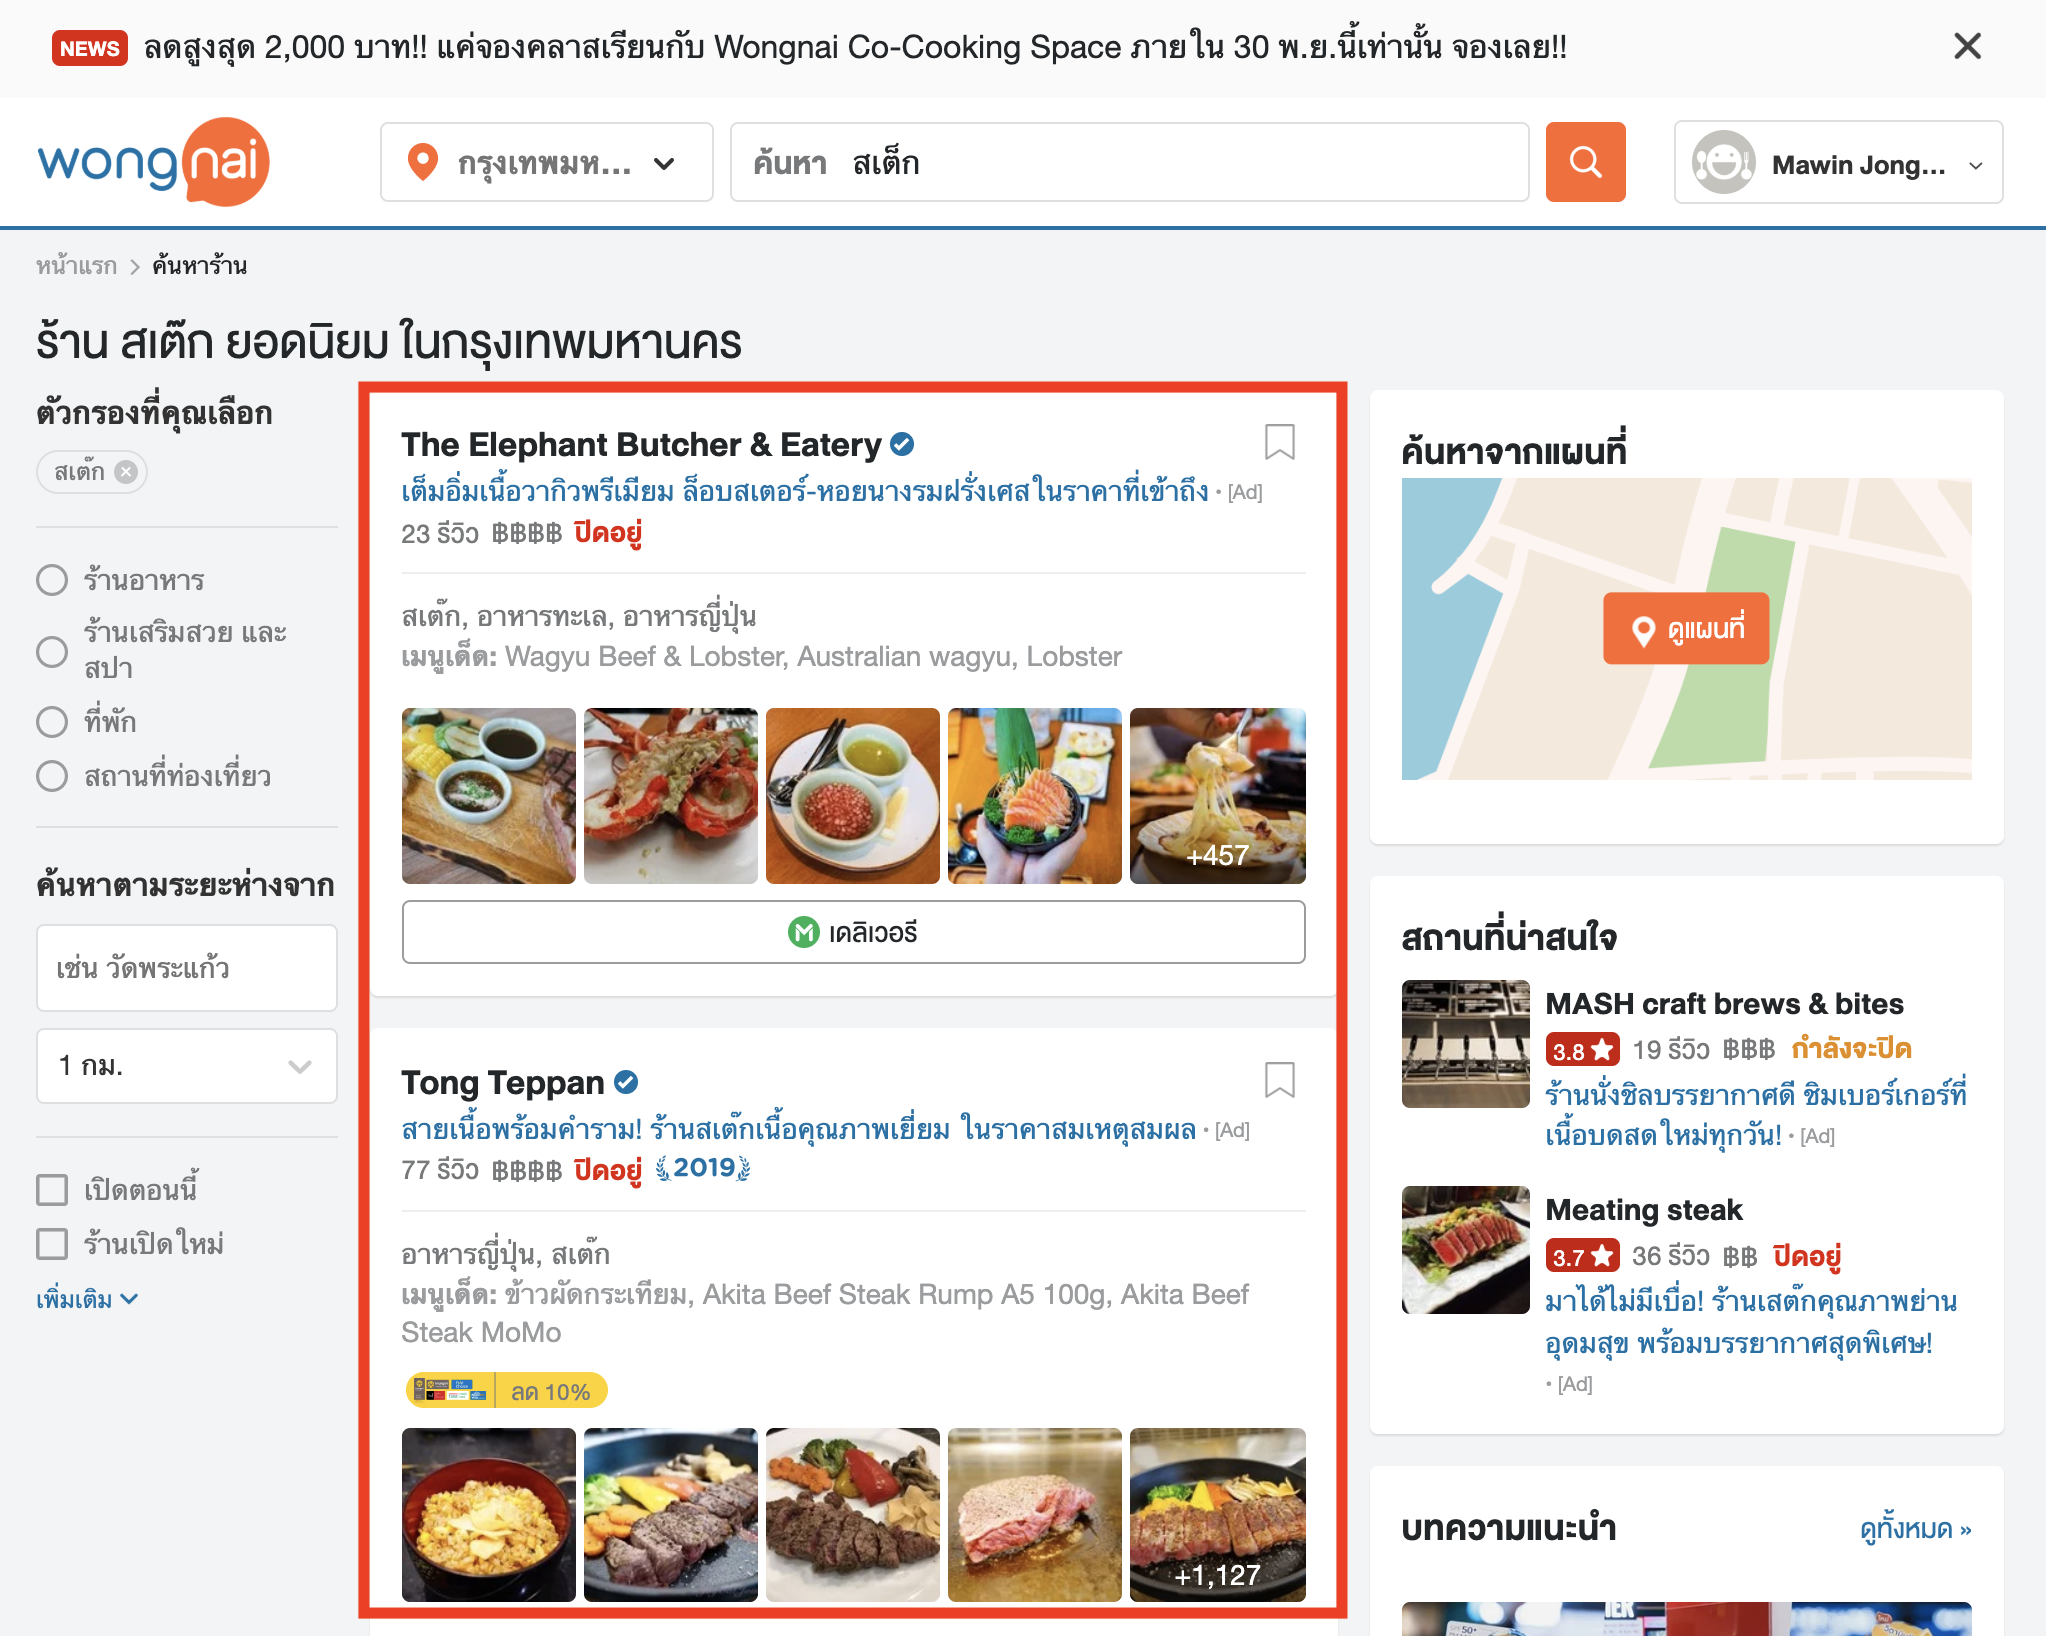
\includegraphics[width=0.8\textwidth]{listing-ad-web.png}  
	}
	\subfigure[]{
		\label{Fig:listingad:ios}
		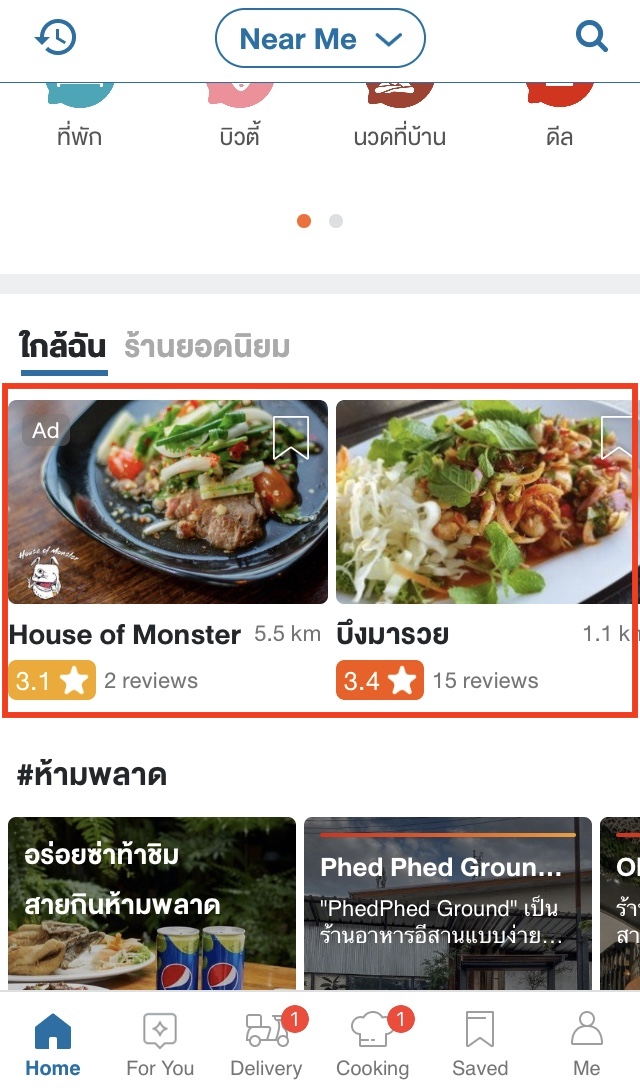
\includegraphics[width=0.4\textwidth]{listing-ad-ios.jpeg}  
	}
	\subfigure[]{
		\label{Fig:listingad:android}
		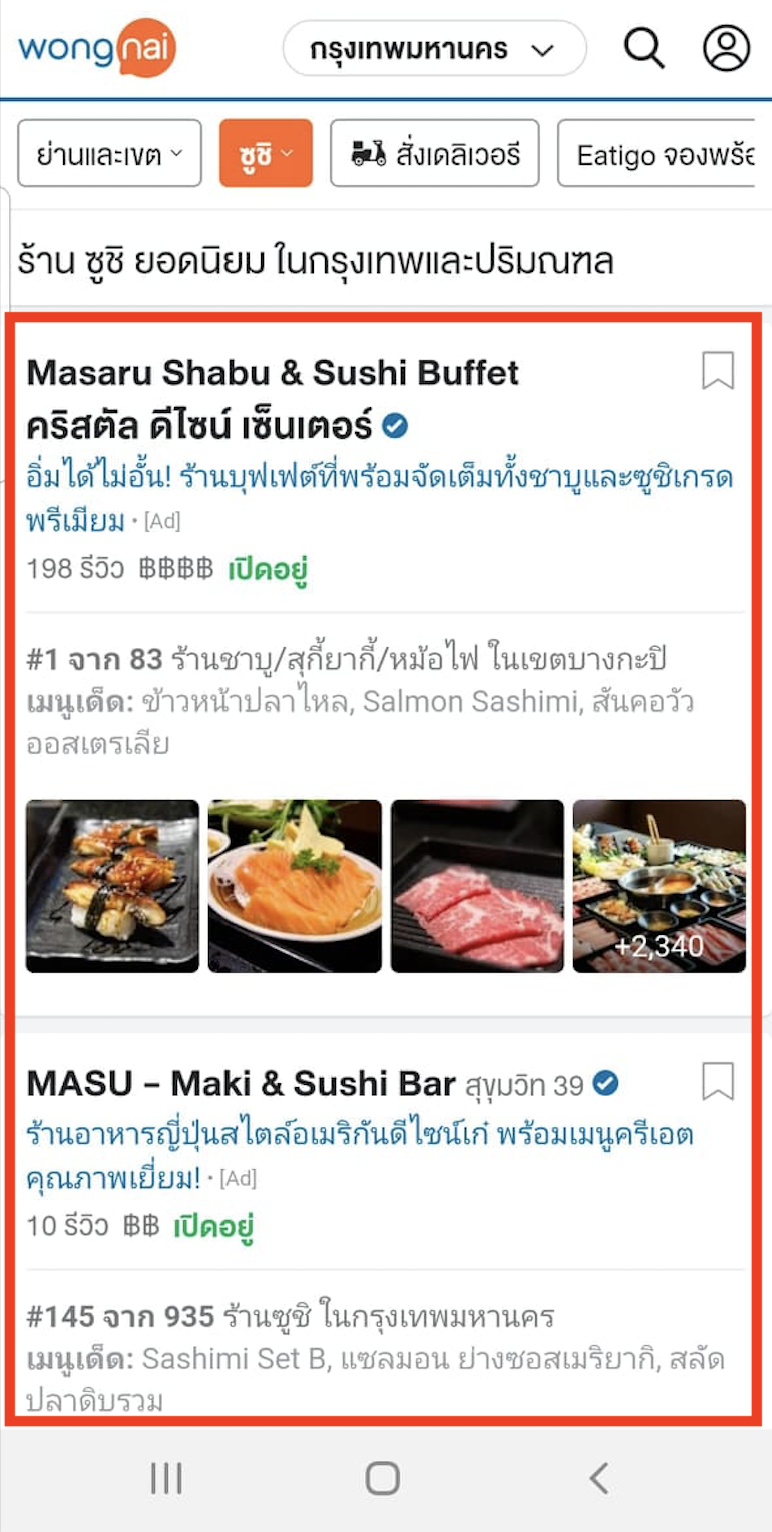
\includegraphics[width=0.35\textwidth]{listing-ad-android.png}  
	}
	\caption{ตัวอย่างการแสดงโฆษณาร้านบนเว็บไซต์ wongnai.com (ก) และบนแอปพลิเคชัน Wongnai ระบบปฏิบัติการ iOS (ข) กับ Android (ค)}
	\label{Fig:listingad}
\end{figure}

\section{วัตถุประสงค์การปฏิบัติงาน}
\begin{enumerate}
	\item เพื่อพัฒนาระบบจัดการโฆษณาแบบจำกัดจำนวนการคลิกและการแสดงโฆษณาที่สามารถใช้งานได้จริง
	\item เพื่อเรียนรู้และหาประสบการณ์ใหม่ ๆ เกี่ยวกับงานด้านวิศวกรรมซอฟต์แวร์โดยการลงมือปฏิบัติงานจริง
	\item เพื่อเรียนรู้และปรับตัวเข้ากับสังคมการทำงาน
\end{enumerate}

\section{ประวัติและรายละเอียดบริษัท}
บริษัท วงใน มีเดีย จำกัด (สำนักงานใหญ่) ตั้งอยู่ที่ อาคารทีวัน ชั้น 26, 27 ซอยสุขุมวิท 40 แขวงพระโขนง เขตคลองเตย กรุงเทพมหานคร 10110 ก่อตั้งเมื่อปี พ.ศ. 2553 เป็นองค์กรที่ให้บริการเว็บไซต์ wongnai.com และแอปพลิเคชัน Wongnai ทั้งบนระบบปฏิบัติการ Android และ iOS ซึ่ง Wongnai นั้น ได้รับการยอมรับว่า เป็นแอปพลิเคชันค้นหาร้านอาหารอันดับ 1 ของไทยที่มีข้อมูลมากที่สุด ครอบคลุมทั้งร้านอาหาร, ร้านเสริมสวย, สปา, สูตรอาหาร, โรงแรม, ที่พัก และที่เที่ยว ปัจจุบัน Wongnai เป็นผู้นำตลาดระบบรีวิวร้านอาหารในไทย โดยมีจำนวนผู้ใช้กว่า 8 ล้านรายต่อเดือน มีฐานข้อมูลมากกว่า 230,000 ร้านทั่วประเทศไทยที่อัพเดทตลอดเวลา รวมทั้งยังได้รับข้อมูลที่ถูกต้องและรีวิวที่มาจากผู้ที่ไปใช้บริการมาจริงเพื่อช่วยประกอบการตัดสินใจ จากสมาชิกที่มีมากกว่า 3 ล้านคนทั่วประเทศ Wongnai มีเป้าหมายหลัก คือ ต้องการที่จะเชื่อมต่อคนไทยเข้ากับสิ่งดี ๆ ทุกอย่างไม่ว่าจะเป็นร้านอาหารร้านเสริมสวยและธุรกิจบริการอื่น ๆ

\begin{figure}[!h]
	\centering
	
\includegraphics[width=0.8\textwidth]{wongnai-logo.png}  
	\caption{ตราสัญลักษณ์ของ Wongnai}
	\label{Fig:wongnai-logo}
\end{figure}